Each of the models presented indicate that the GSN framework is suitable for learning useful representations of complex sequential input data. The results are summarized below and compared to the RNN-RBM model discussed in Chapter 2 (Related Work):

\begin{table}[h!]
\begin{tabular*}{\textwidth}{p{4cm} r r r r}
\hlinewd{1.5pt}
  & Model 1 & Model 2 & Model 3 & RNN-RBM \\
\hline
Reconstruction binary cross-entropy & 0.2317 & 0.2318 & (waiting for results) & 0.2173\\
\hlinewd{1.5pt}
\end{tabular*}
\caption{Binary cross-entropy of the predicted sequence reconstruction comparison of the 3 models and an RNN-RBM on artificially sequenced (0-9 repeating) MNIST data.}
\end{table}

While binary cross-entropy is a useful metric for the reconstruction error, it does not necessarily indicate quality of visual reconstruction (as seen by the generative samples). While each model has a similar cross-entropy score, they produce quite different reconstructions of corrupted input data. These generative samples show what each model is encoding from the input space:

\begin{itemize}
	\item Model 1 learns a good representation of the current input and a transition to the average value of the predicted next input.
	\item Model 2 learns a representation mixing between the modes of the sequence over the input data.
	\item Model 3 learns a good representation of the current input as well as a good representation of the sequence of representations given the input data.
\end{itemize}

Compared to the samples generated by the RNN-RBM, it is clear that the GSN framework has an easier time mixing between modes of the input data. It also appears to form better reconstructions of the input data. This improvement can be attributed to a deeper representation of the input space, since the RNN-RBM only had two layers - one for the RBM and one for the RNN.

\begin{figure}[h!]
  \centering
    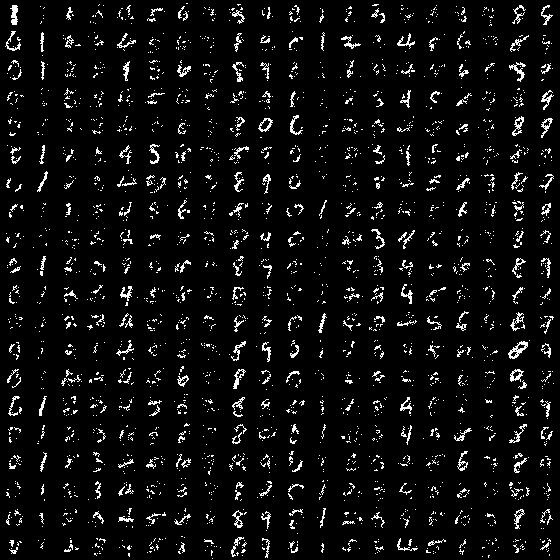
\includegraphics[width=0.8\textwidth]{rnnrbm_samples}
\caption{RNN-RBM sampling after 300 iterations.}
\end{figure}